
\section{Misconceptions in Some Existing Results}

\subsection{Incorrect Quantifications of Jitter - Dynamic Self-Suspension}
\label{sec:wrong-jitter-dynamic}

We first explain the existing misconceptions in the literature to quantify the jitter too optimistically for dynamic self-suspending task systems. To calculate the worst-case response time of the task $\tau_k$ under analysis, there have been several results in the literature, i.e., \cite{ECRTS-AudsleyB04,RTAS-AudsleyB04,RTCSA-KimCPKH95},  which propose to calculate the worst-case response time of task $\tau_k$ by finding the minimum $R_k$ with
\begin{equation}
R_k = C_k+ S_k+\sum_{\tau_i \in hp(k)}\ceiling{\frac{R_k+S_k}{T_i}} C_i.
\label{eq:dynamic-flawed}
\end{equation}
The term $hp(k)$ is the set of higher-priority tasks for $\tau_k$. This analysis basically assumes that the jitter of a higher-priority task $\tau_i$ due to self-suspension is at most $S_i$.  Intuitively, it represents the potential internal jitter, \textit{within} an activation of $\tau_i$, i.e., when its execution time $C_i$ is considered by disregarding any time intervals when $\tau_i$ is preempted. 
However, it is not a real jitter in the general case, because the execution of $\tau_i$ can be pushed further to the right. 


Consider the dynamic self-suspending task set presented in Table \ref{tab:counterexample-dynamic-suspension}. 
The analysis in Eq.~(\ref{eq:dynamic-flawed}) would yield $R_3=12$, as illustrated in 
Figure~\ref{fig:counterexample-dynamic}(a). However, the schedule of Figure~\ref{fig:counterexample-dynamic}(b), which is perfectly legal, 
disproves the claim that $R_3=12$, because $\tau_3$ in that case has a response time of $32-5\epsilon$ time units, 
where $\epsilon$ is an arbitrarily small quantity. 

\begin{table}[t]
\begin{center}
\begin{tabular}{|c|r|r|r|}
\hline
$\tau_i$ &      $C_i$   &   $S_i$  &     $T_i$     \\ \hline
$\tau_1$ &       $1$   &     $0$  &       $2$     \\ \hline
$\tau_2$  &      $5$   &     $5$  &      $20$     \\ \hline
$\tau_3$  &      $1$   &     $0$  &  $\infty$     \\ \hline
\end{tabular}
\end{center}
\caption{A set of tasks with self-suspensions.}
\label{tab:counterexample-dynamic-suspension}
\end{table}

\begin{figure}[t]
\begin{center}
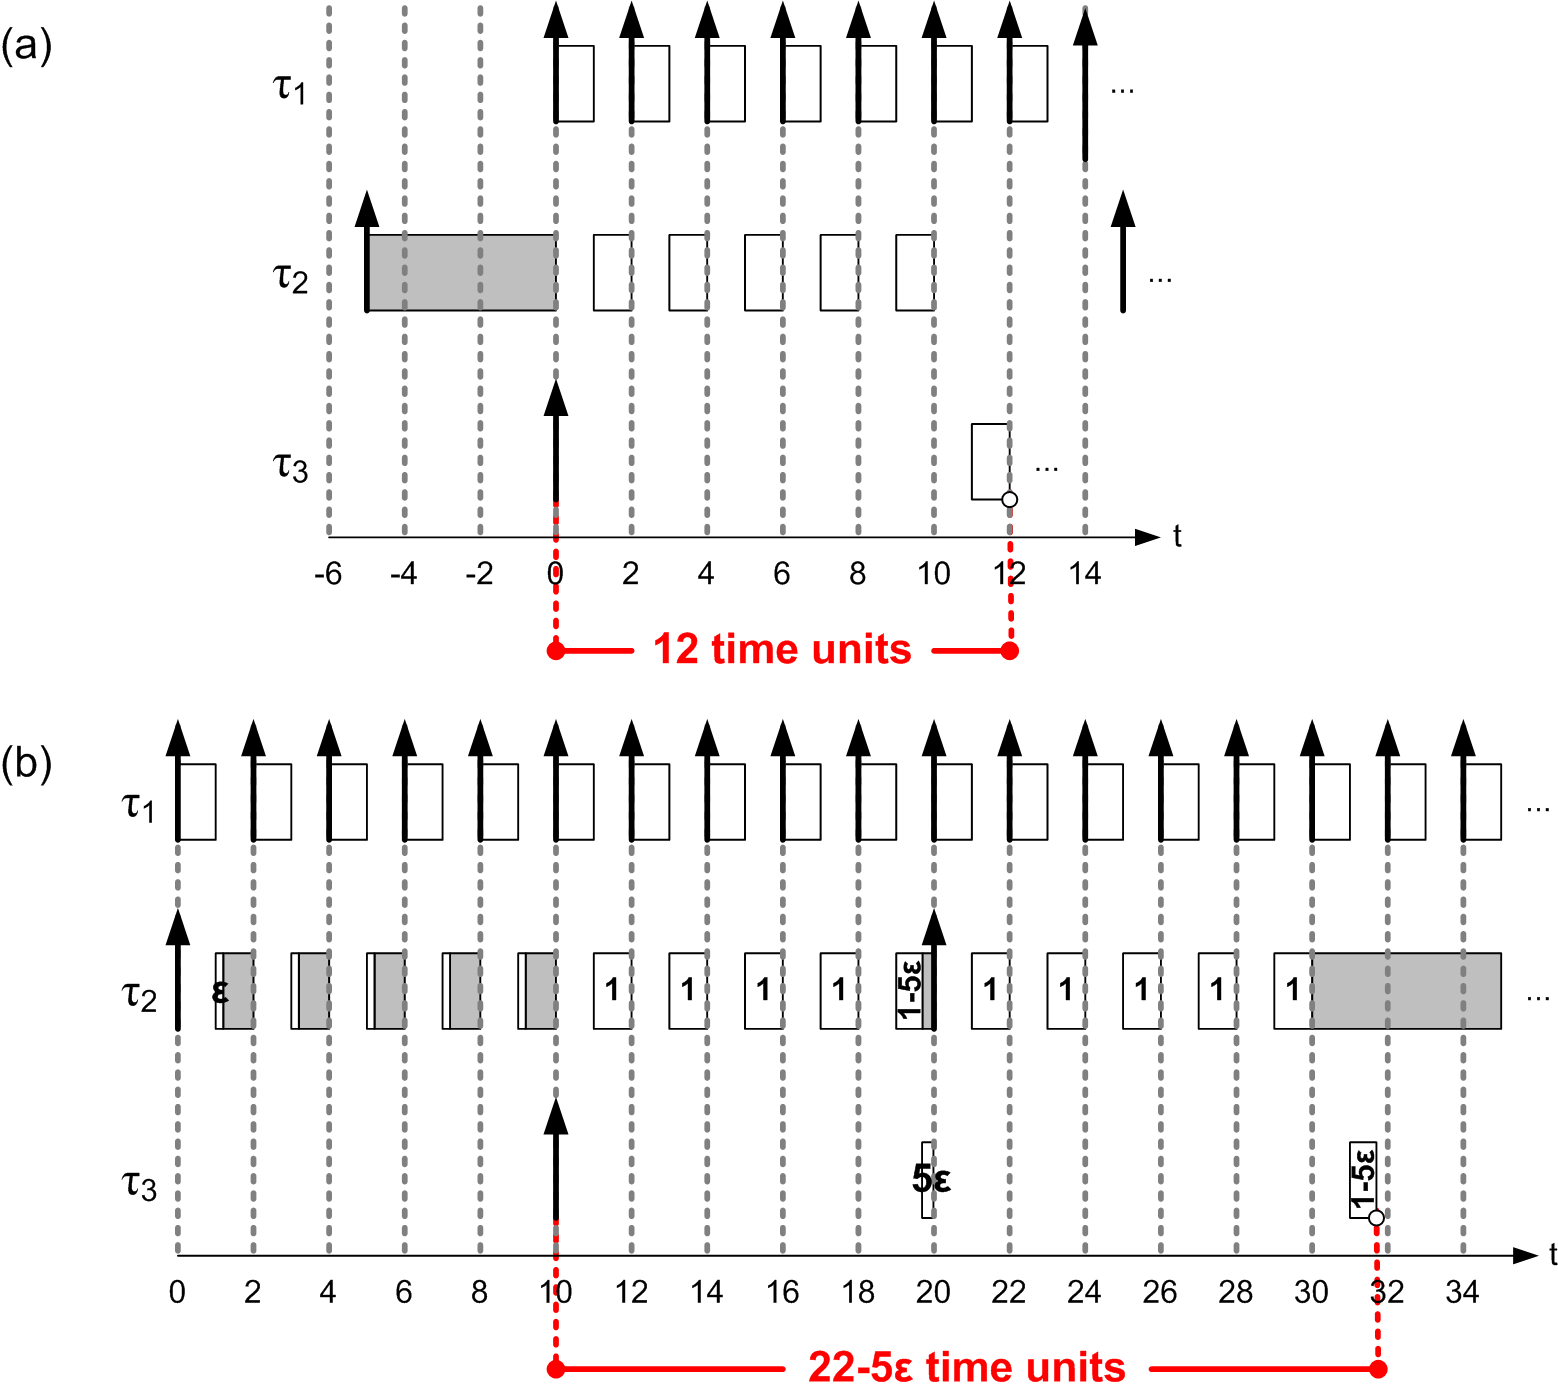
\includegraphics[width=\linewidth]{../figures/CounterexampleDynamicSuspension/counterexample_classic.png}
\end{center}
\caption{Two different schedules for the task set in Table~\ref{tab:counterexample-dynamic-suspension}.}
\label{fig:counterexample-dynamic}
\end{figure}

{\bf Consequences:} Since the results in \cite{ECRTS-AudsleyB04,RTAS-AudsleyB04,RTCSA-KimCPKH95} are fully based on the analysis in Eq.~(\ref{eq:dynamic-flawed}), the above unsafe example disproves the correctness of their analyses. The authors of the results in \cite{ECRTS-AudsleyB04,RTAS-AudsleyB04} already filed a technical report \cite{BletsasReport2015} to explain in a great detail how to handle this. This misconception was unfortunately picked in \cite{lakshmanan-2009} to analyze the worst-case response time for
partitioned multiprocessor real-time locking protocols, and reused in several other works~\cite{zeng-2011,bbb-2013,yang-2013,kim-2014,han-2014,carminati-2014,yang-2014}. Therefore, this misconception also causes analytical flaws in the above papers. We will explain such consequences in Section~\ref{sec:syn}.
Moreover this counterexample also invalidates the comparison in \cite{RidouardR06}, which compares the feasibility tests from \cite{RTCSA-KimCPKH95} and \cite[Page 164-165]{Liu:2000:RS:518501}, since the result derived from \cite{RTCSA-KimCPKH95} is unsafe.

{\bf Solutions:} It is explained and proved in \cite{huangpass:dac2015} that the worst-case response time of task $\tau_k$ is the minimum $R_k$ with
\begin{equation}
R_k = C_k+ S_k+\sum_{\tau_i \in hp(k)}\ceiling{\frac{R_k+D_i-C_i}{T_i}} C_i,
\label{eq:dynamic-correct}
\end{equation}
for \emph{constrained-deadline} task systems under the assumption that every higher priority task $\tau_i$ in $hp(k)$ can meet their relative deadline constraint. 

\subsection{Incorrect Quantifications of Jitter - Segmented Self-Suspension}
\label{sec:wrong-jitter-segmented}


We then explain the existing misconceptions in the literature to quantify the jitter too optimistically for segmented self-suspending task systems.  The analysis in \cite{RTCSA-BletsasA05} adopts two steps: (1) the computation segments and the self-suspension intervals are reordered such that the computation segments are with decreasing execution time and the suspension interval are with increasing self-suspending time; and (2) each computation segment has a constant jitter defined by the \emph{early completion of the computation segments and the self-suspension intervals} prior to this computation segment, regardless of other tasks. 

Instead of going into the detailed mathematical formulations, we will demonstrate the above misconception with the following example listed in Table~\ref{tab:counterexample-segmented}.
In this example, there is only one self-suspending task $\tau_3$. Suppose that all the values of computation time and self-suspension time are all for the actual-case costs. Therefore, both steps mentioned above do not take any effect. The analysis in \cite{RTCSA-BletsasA05} is basically akin to replacing $\tau_3$ with a sporadic task without any jitter or self-suspension, with $C_3=2$ and $D_3=T_3=15$. Therefore, the analysis in \cite{RTCSA-BletsasA05}  concludes that the worst-case response time of task $\tau_4$ is at most $15$ since $C_4+\sum_{i=1}^{3}\ceiling{\frac{15}{T_i}} C_i = 3+ 6 + 4 + 2= 15$.


However, the schedule of Figure \ref{fig:counterexample-segmented} which is perfectly legal, disproves this.
In that schedule, $\tau_1$, $\tau_2$, and $\tau_3$ arrive at $t=0$ and a job by $\tau_4$ arrives at $t=40$ and has a response time of 
$18$ time units.

\begin{table}[t]
\begin{center}
\begin{tabular}{|c||c|r|r|r|}
\hline
$\tau_i$ & $(C_i^1, S_i^1, C_i^2)$   &   $D_i$  &     $T_i$     \\ \hline
$\tau_1$ &  $(2, 0, 0)$                    &     $5$  &       $5$     \\ \hline
$\tau_2$ &  $(2, 0, 0)$                    &    $10$  &      $10$     \\ \hline
$\tau_3$ &  $(1, 5, 1)$            &    $15$  &      $15$     \\ \hline
$\tau_4$ &  $(3, 0, 0)$                   &    $?$  &   $\infty$    \\ \hline     
\end{tabular}
\end{center}
\caption{A set of segmented self-suspending and sporadic real-time tasks.}
\label{tab:counterexample-segmented}
\end{table}




\begin{figure}[t]
\begin{center}
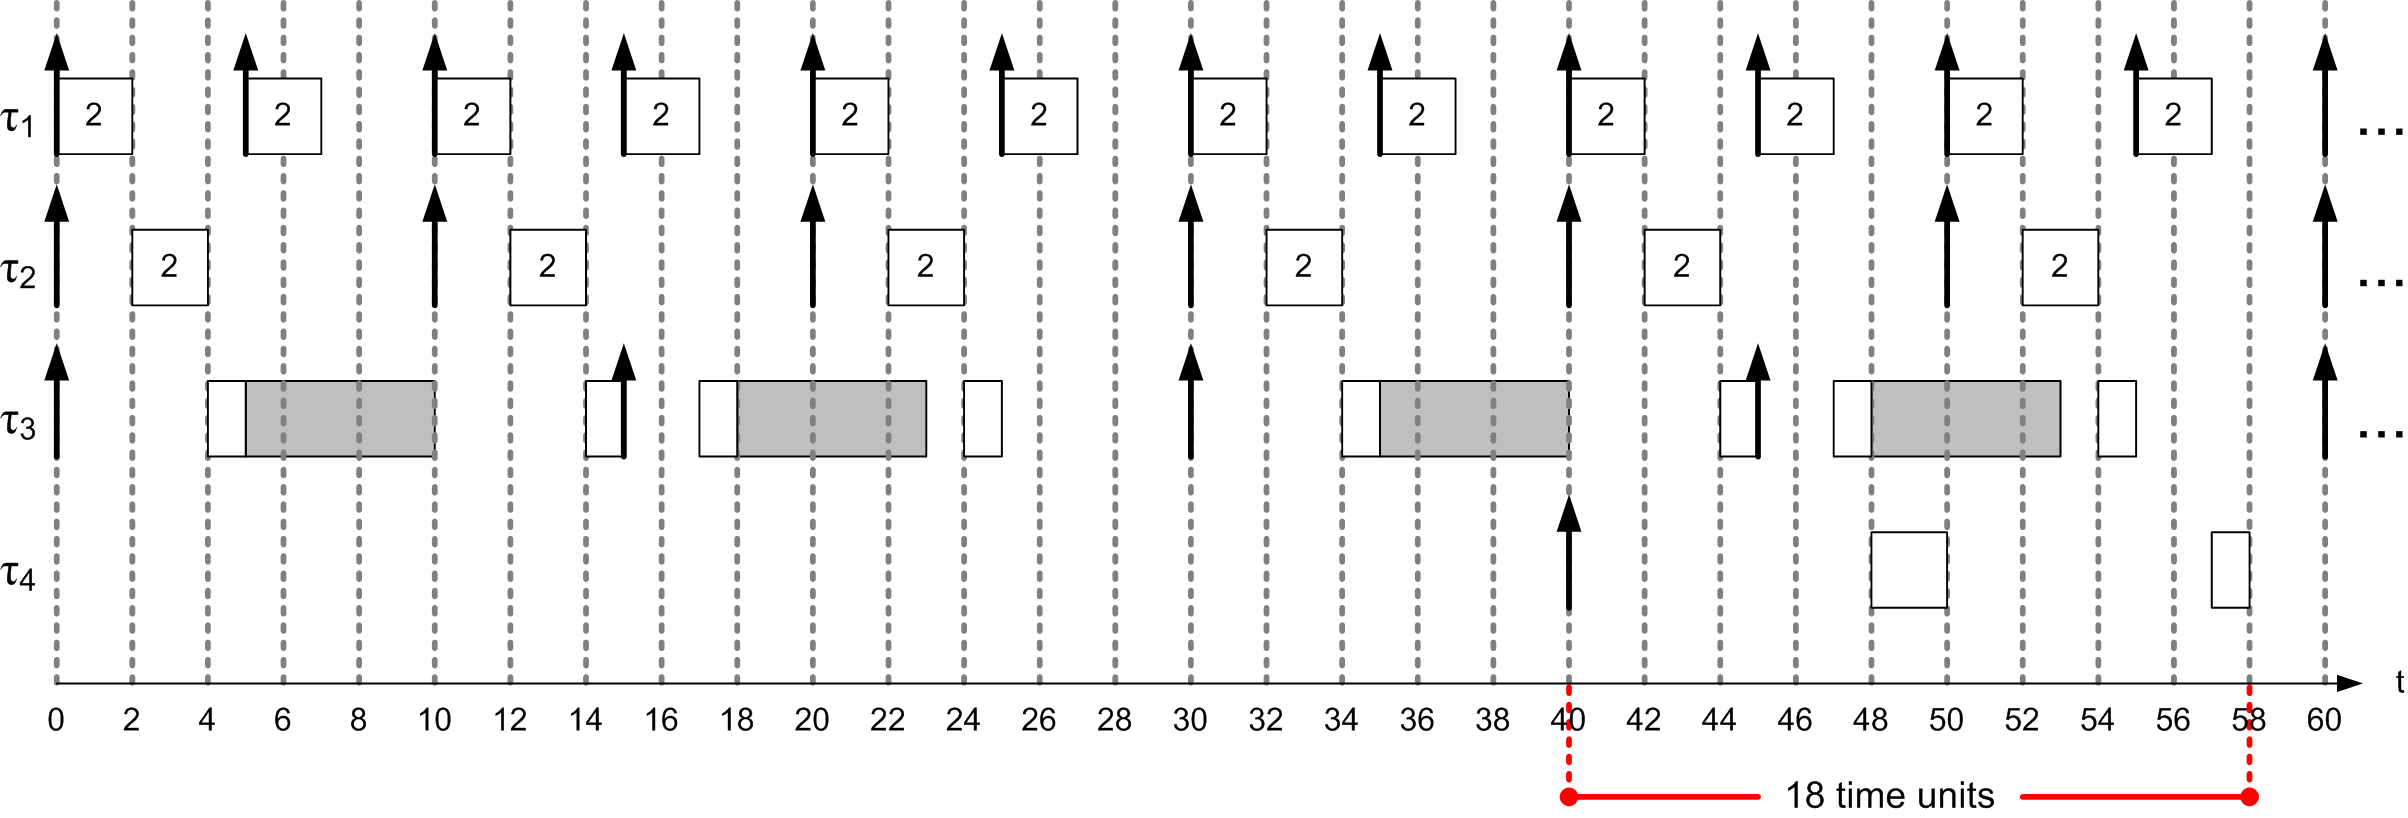
\includegraphics[width=\linewidth]{../figures/CounterexampleSegmentedSuspension/counterexample_synthetic.png}
\end{center}
\caption{A schedule for the task set in Table  \ref{tab:counterexample-segmented}. }
\label{fig:counterexample-segmented}
\end{figure}


{\bf Consequences:} This example shows that the analysis in \cite{RTCSA-BletsasA05} is flawed.  The authors in \cite{RTCSA-BletsasA05}  already filed a technical report \cite{BletsasReport2015}.

{\bf Solutions:} There is no simple way to fix the error, but quantifying the jitter of a self-suspending task $\tau_i$ with $D_i-C_i$ in Section~\ref{sec:wrong-jitter-dynamic}  remains safe since the dynamic self-suspending pattern is more general than a segmented self-suspending pattern.

\subsection{Incorrect Assumptions in Critical Instant Theorem with Synchronous Releases}
\label{sec:wrong-critical}

Over the years, it has been well accepted that the characterization of the critical instant for self-suspending tasks is a complex problem. Nevertheless, although the complexity of verifying the existence of a feasible schedule for segmented self-suspending tasks has been proven to be ${\cal NP}$-hard in the strong sense \cite{Ridouard_2004}, the complexity of verifying the schedulability of a task set has only been studied for segmented self-suspending tasks with constrained deadlines scheduled with a fixed-priority scheduling algorithm (see Section~\ref{sec:hardness}), hence leaving hope for the existence efficient schedulability tests for more constrained systems. 

Following that idea, Lakshmanan and Rajkumar \cite{LR:rtas10} propose a pseudo-polynomial worst-case response time analysis for one segmented self-suspending (with one self-suspending interval) task $\tau_k$ assuming that 
\begin{itemize}
\item the scheduling algorithm is fixed priority (FP);
\item $\tau_k$ is the lowest priority task; 
\item all the higher priority tasks are sporadic;
\item all the higher priority tasks are non-self-suspending.
\end{itemize}
The analysis, presented \cite{LR:rtas10}, is based on the notion of critical instant, i.e., an instant at which, considering the state of the system, an execution request for $\tau_k$ will generate the largest response time. This critical instant was defined as follows:
\begin{itemize}
	\item every task releases a job simultaneously with $\tau_k$;
	\item the jobs of higher priority tasks that are eligible to be released during the self-suspension interval of $\tau_k$ are delayed to be aligned with the release of the subsequent computation segment of $\tau_k$; and
	\item all the remaining jobs of the higher priority tasks are released with their minimum inter-arrival time.
\end{itemize}

This definition of the critical instant is very similar to the definition of the critical instant of a non-self-suspending task. Specifically, it is based on the two intuitions that $\tau_k$ suffers the worst-case interference when (i) all higher priority tasks release a job simultaneously with $\tau_k$ and (ii) they all release as many jobs as possible in each computation segment of $\tau_k$. Although intuitive, we provide examples that both statements are wrong\footnote{Note that both examples were already published in \cite{ecrts15nelissen}.}.

\subsubsection{A Counter-Example to the Synchronous Release}

\begin{table} 
\centering
    \begin{tabular}{|c|c|c|}
 \hline
        & $(C_i^1, S_i^1, C_i^2)$ &  $D_i=T_i$\\ 
        \hline
        $\tau_1$ & (1, 0, 0) &  4\\ 
        $\tau_2$ &  (1, 0, 0) & 50  \\ 
        $\tau_3$ & (1, 2, 3) & 100  \\
        \hline
    \end{tabular} 
    \caption{Task parameters for the counter-example to the synchronous release of all tasks.}
    \label{table:ex-synch-releases}
\end{table}

\ifpaper
\begin{figure}[t]
  \centering
\captionsetup[subfigure]{width=\columnwidth}
  \subfloat[all tasks release a job synchronously.]{\label{fig:ex-phi} }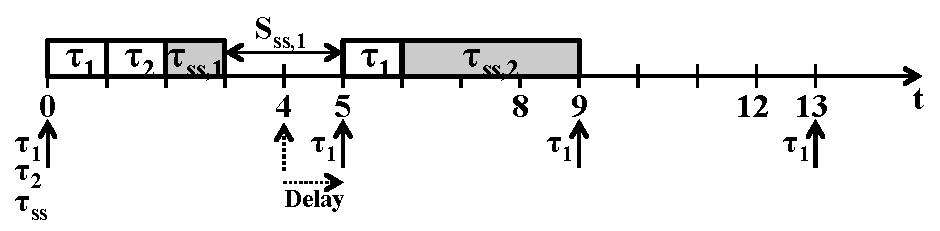
\includegraphics[width=0.85\linewidth]{../figures/ex-phi/ex-phi.pdf} \\
  \subfloat[all tasks do not release a job synchronously.]{\label{fig:ex-no-phi} }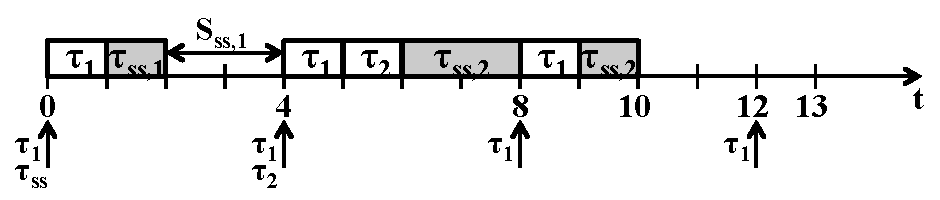
\includegraphics[width=0.85\linewidth]{../figures/ex-no-phi/ex-no-phi}
  \caption{Counter-example to the synchronous release of all tasks (by \cite{LR:rtas10}).}
  \label{fig:ex-synch-releases}
\end{figure}
\fi

Consider three implicit deadline tasks with the parameters presented in Table~\ref{table:ex-synch-releases}. Let us assume that the priorities of the tasks are assigned using the rate monotonic policy (i.e., the smaller the period, the higher the priority). We are interested in computing the worst-case response time of $\tau_3$. Following the definition of the critical instant presented in \cite{LR:rtas10}, all three tasks must release a job synchronously at time $0$. Using the standard response-time analysis for non-self-suspending tasks, we get that the worst-case response time of the first computation region of $\tau_3$ is equal to $R_3^1 = 3$. Because the second job of $\tau_1$ would be released in the self-suspending interval of $\tau_3$ if $\tau_1$ was strictly respecting its minimum inter-arrival time, the release of the second job of $\tau_1$ is delayed so as to coincide with the release of the second computation region of $\tau_3$ (see Figure~\ref{fig:ex-phi}). Considering the fact that the second job of $\tau_2$ cannot be released before time instant $50$ and hence does not interfere with the execution of $\tau_3$, the response time of the second computation segment of $\tau_3$ is thus equal to $R_3^2=4$. In total, the worst-case response time of $\tau_3$ when all tasks release a job synchronously is equal to 
$$R_3 = R_3^1 + S_3^1 + R_3^2 = 3 + 2 +4 = 9$$

Now, let us consider a job release pattern as shown in Figure~\ref{fig:ex-no-phi}. Task $\tau_2$ does not release a job synchronously with task $\tau_3$ but with its second computation segment instead. The response time of the first computation segment of $\tau_3$ is thus reduced to $R_3^1=2$. However, both $\tau_1$ and $\tau_2$ can now release a job synchronously with the second computation segment of $\tau_3$, for which the response time is now equal to $R_3^2=6$ (see Fig.~\ref{fig:ex-no-phi}). Thus, the total response time of $\tau_3$ in a scenario where not all higher priority tasks release a job synchronously with $\tau_3$ is equal to 
$$R_3 = R_3^1 + S_3^1 + R_3^2 = 2+2+6 = 10$$

To conclude, the synchronous release of all tasks does not necessarily generate the maximum interference for the self-suspending task $\tau_k$ and is thus not always a critical instant for $\tau_k$. It was however proven in \cite{ecrts15nelissen} that in the critical instant of a self-suspending task $\tau_k$, every higher priority task releases a job synchronously with the arrival of at least one computation segment of $\tau_k$, but not all higher priority tasks must release a job synchronously with the same computation segment.



\subsection{Counting Highest-Priority Self-Suspending Time to Reduce the Interference}
\label{sec:wrong-highest-priority}

We now present a misconception to handle the highest-priority segmented self-suspension task by using the self-suspension time to reduce its interference to the lower-priority sporadic task systems. 
We consider fixed-priority preemptive scheduling to schedule $n$ self-suspending sporadic real-time tasks on a single processor, in which $\tau_1$ is the highest priority task and $\tau_n$ is the lowest priority task. We focus on constrained-deadline task systems with $D_i \leq T_i$ or implicit-deadline systems with $D_i=T_i$ for $i=1,\ldots,n$.
Let's consider the simplest setting of such a case:
\begin{itemize}
\item there is only one self-suspending task, which is the highest-priority task, i.e., $\tau_1$,
\item the self-suspending time is fixed, i.e., early return of self-suspension has to be controlled, and
\item the actual execution time of the self-suspending task is always equal to the worst-case execution time.
\end{itemize}
Such a task set (system) is referred to as $\Gamma_{1s}$.  Since $\tau_1$ is the highest-priority task, its execution behaviour is static under the above assumptions. The misconception here is to identify the critical instant  (Theorem 2 in \cite{RTSS-KimANR13}) as follows: ``a critical instant occurs when all the tasks are released at the same time if $C_1 +S_1 < C_i  \leq T_1-C_1-S_1 \mbox{ for } i \in\{i|i\in Z^{+} \mbox{ and } 1<i\leq n\}$ is satisfied.'' The misconception here is to use the self-suspension time (if it is long enough) to \emph{reduce} the computation demand of $\tau_i$ for interfering the lower-priority tasks. 


{\it Counterexample of Theorem 2 in \cite{RTSS-KimANR13}:} Let $\epsilon$ be a positive and very small number, i.e., $0 < \epsilon \leq 0.1$. We have $3$ tasks, in which
(1) $C_1= 1+ \epsilon$, $C_1^1 = \epsilon$, $S_1=S_1^1 = 1$, $C_1^2  = 1$, $T_{1} =D_1= 4 + 10 \epsilon$, (2) $C_2 = 2 + 2\epsilon$, $T_2 =D_2= 6$, and (3)
$C_3 = 2 + 2\epsilon$, $T_3 =D_3= 6$. It is clear that $2+\epsilon = C_1+S_1 < C_i = 2+2\epsilon \leq T_1-C_1-S_1 = 2+9\epsilon$ for $i=2,3$. The above theorem states that the worst case is to release all the three tasks together at time $0$. The analysis shows that the response time of task $\tau_3$ is at most $5+6\epsilon$. However, if we release task $\tau_1$ at time $0$ and release task $\tau_2$ and task $\tau_3$ at time $1+\epsilon$, the response time of the first job of task $\tau_3$ is $6+5\epsilon$. 

This misconception also leads to a wrong statement in Theorem 3 in \cite{RTSS-KimANR13}:
\begin{quote}
{\it Theorem 3 in \cite{RTSS-KimANR13}}: For a taskset $\Gamma_{1s}$ with implicit deadlines, $\Gamma_{1s}$ is schedulable if the total utilization of the taskset is less than or equal to $n((2+2\gamma)^{\frac{1}{n}}-1)-k$, where $n$ is the number of tasks in $\Gamma_{1s}$, and $\gamma$ is the ratio of
$S_1$ to $T_1$ and lies in the range of $0$ to $2^{\frac{1}{n-1}}-1$. 
\end{quote}


{\it Counterexample of Theorem 3 in \cite{RTSS-KimANR13}:} Suppose that the self-suspending task $\tau_1$ has two computation segments, with $C_1^1 = C_1-\epsilon$, $C_1^2 = \epsilon$, and $S_1=S_1^1 > 0$ with very small $0 < \epsilon \ll C_1^1$. For such an example, it is pretty trivial that this self-suspending highest-priority task is like a sporadic task, i.e., self-suspending does not matter. 

{\bf Consequences:} These examples show that Theorems 2 and 3 in \cite{RTSS-KimANR13} are flawed.  

{\bf Solutions:} The three assumptions, i.e., one highest-priority segmented self-suspending task, controlled suspension behaviour and controlled execution time  in \cite{RTSS-KimANR13} actually implies that the self-suspending behaviour of task $\tau_1$ can be modeled as sporadic events with minimum inter-arrival time. That is, if the $j$-th computation segment of task $\tau_1$ starts its execution at time $t$, the earliest time for this computation segment to be executed again in the next job of task $\tau_1$ is at least $t+T_1$. Therefore, a constrained-deadline task $\tau_k$ can be feasibly scheduled by the fixed-priority scheduling strategy if $C_1+S_1 \leq D_1$ and for $2 \leq k \leq n$
  \begin{equation}
    \label{eq:tda-fixed}
\exists 0 < t \leq D_k, \qquad C_k + \sum_{i=1}^{k-1}\ceiling{\frac{t}{T_i}}C_i \leq t.    
  \end{equation}
This also implies that the utilization bound (for implicit-deadline task systems) is still Liu and Layland bound $n(2^{\frac{1}{n}}-1)$ \cite{Liu_1973}, regardless of the ratio of $S_1/T_1$. 

\subsection{Incorrect Scheduling with Periodic Execution Enforcement}
\label{sec:wrong-periodic}

We now introduce another misconception. 



%%% Local Variables:
%%% mode: latex
%%% TeX-master: "JRTS/JRTS.tex"
%%% End:
